\begin{frame}[allowframebreaks]{\underline{Results} -}
    \section{Results}
The problem addressed here involves minimizing $C_d$, subject to constraints as mentioned.
\begin{frame}{\underline{Problem statement}}
\section{Problem statement}
\small{To solve the ADO-DG  (\textit{Aerodynamic Design Optimization and Discussion Group}) case 6: }
\\[2mm]
\begin{itemize}
\item Objective function is to minimize $C_D$
\item $C_L$ = 0.375, Mach = 0.5
\item Baseline geometry NACA 0012 wing with semi span 3.06 units
\item  Intented to have multimodal optima
\item Geometric parameters as described in the problem
\end{itemize}

\parbox{0.38\linewidth}{
\textit\textit{{Result should highlight:}}
\begin{itemize}
\item Number of optima 
\item Geometry description of each optimal wing
\item Evidence for convergence
\item Performance value, $eb^2$, b as final span, and $e$(span efficiency factor) is defined as,
$$\boxed{
e=\frac{C_{L}^{2}}{2 \pi S C_{D}}
}$$
\end{itemize}
}
\parbox{0.57\linewidth}{
\begin{figure}
    \centering
    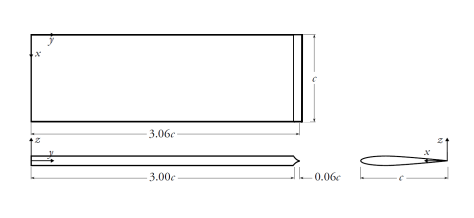
\includegraphics[scale = 0.34]{figures/baselinewing.png}
    \caption{baseline wing}
    \label{fig:baseline wing}
\end{figure}
}

\end{frame}

\underline{Grid sensitivity:}
\begin{table}[!htbp]
    \centering
    \begin{tabular}{|c|c|c|}\hline
        \textbf{Mesh quality} & \textbf{Surface mesh} & \textbf{Volume mesh} \\\hline
        Coarse  & 150 $\times$ 100 & 0.11m \\
        Fine  & 300 $\times$ 200 & 0.25m \\\hline
    \end{tabular}
    \caption{Grid sensitivity analysis}
    \label{grid_sensitivity}
\end{table}

\parbox{0.57\linewidth}{
\begin{figure} 
    \centering
    \framebox{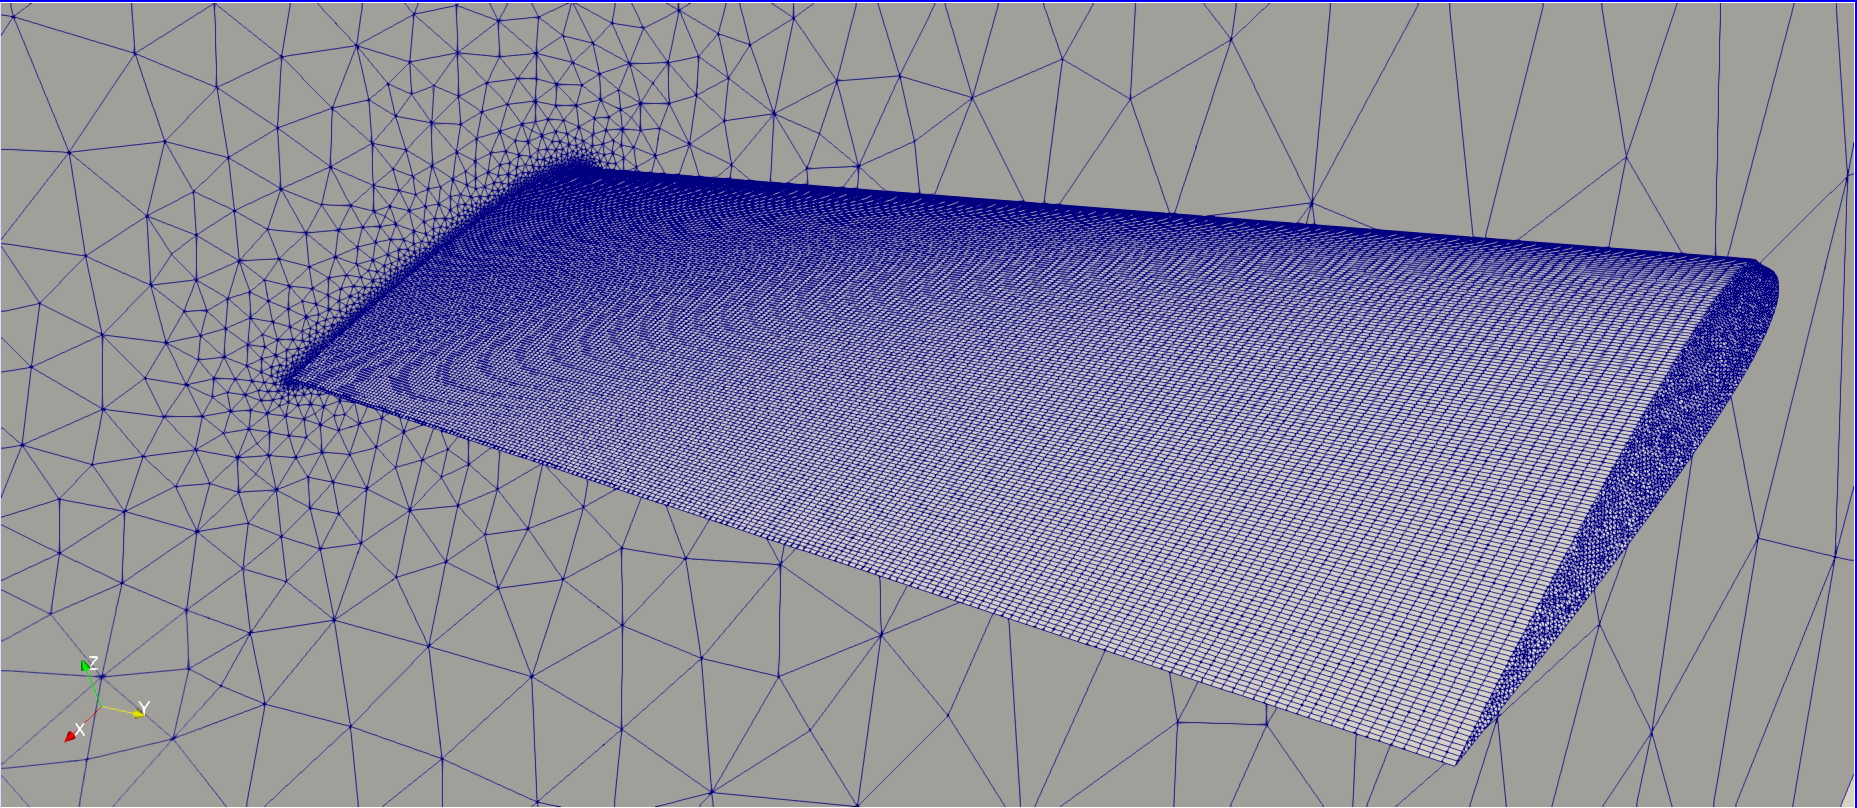
\includegraphics[scale = 0.08]{figures/fine_mesh_wing.png}}
    \caption{Fine mesh with 300 $\times$ 200 surface mesh points.}
    \label{fine_mesh}
\end{figure}
}
\parbox{0.37\linewidth}{
\begin{figure} 
    \centering
    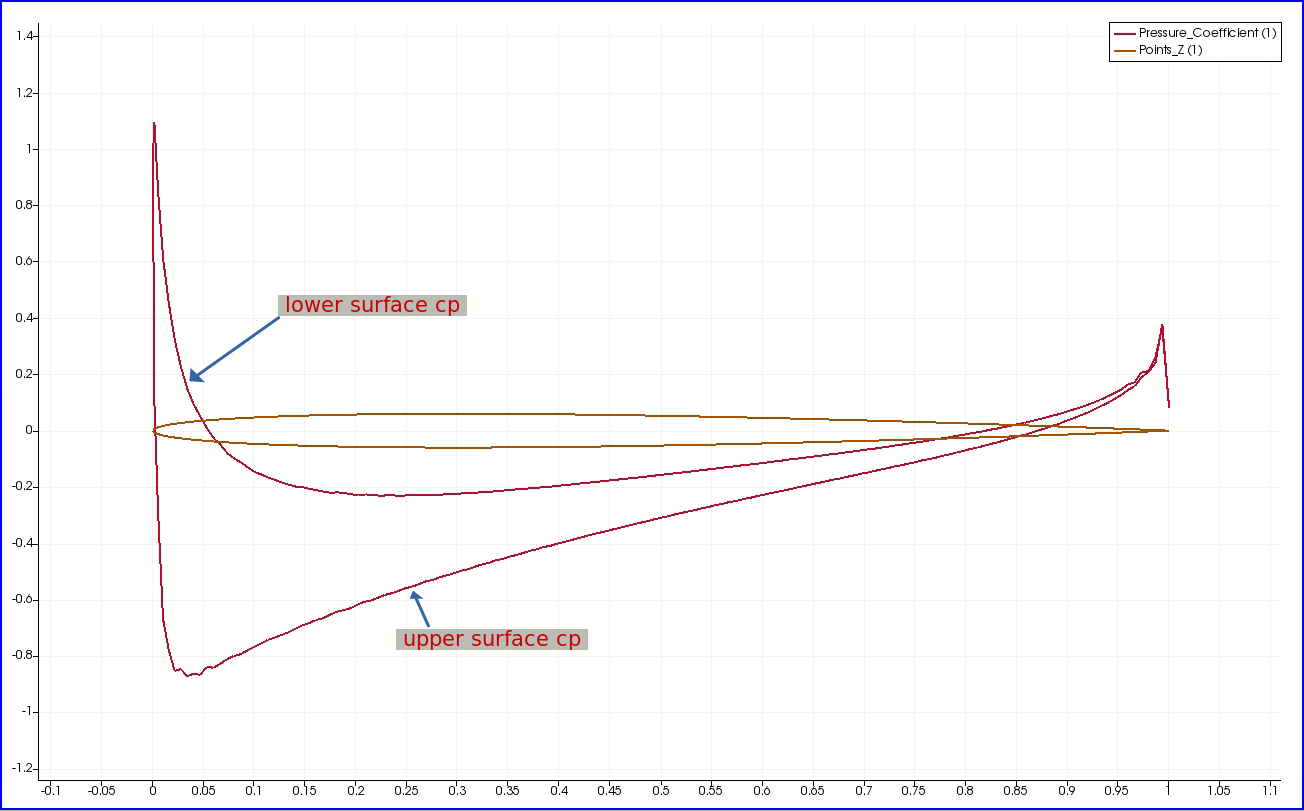
\includegraphics[scale = 0.08]{figures/cp_curve.png}
    \caption{Cp curve at root section of fine mesh (300 $\times$ 200).}
    \label{cp curve}
\end{figure}
}
\begin{itemize}
\item Due to sharp trailing edge, there is some disturbance in the Cp.
\item The fine mesh appears appropriate to proceed with full optimization.
\item The baseline (NACA 0012) geometry has Cd of 5.08 $\times$ $10^{-2}$, with $C_l$ constraint satisfied by adjusting
the angle of attack.
\end{itemize}

\underline{Initial population:}
\begin{figure} 
    \centering
    \framebox{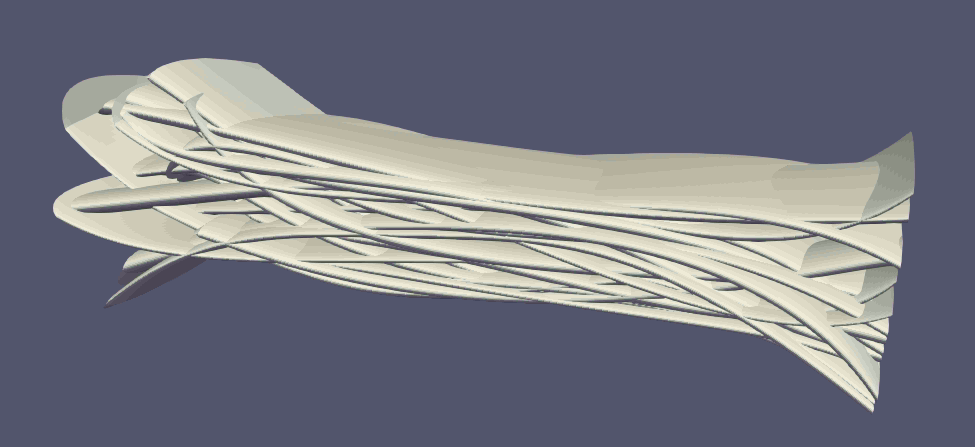
\includegraphics[scale=0.2]{figures/initial_population.png}}
    \caption{Initial 20 populations.}
    \label{initial_population}
\end{figure}
\begin{itemize}
    \item These population cover all the
design space like dihedral, taper wings, sweep backward/forward, winglet up/down, and
span long/short.
\end{itemize}

\underline{Local optima 1:}
\begin{itemize}
\item The Mach number is 0.4.
\item Flow is subsonic and inviscid.
\item The angle of attack is varied between -$3^0$ and +$6^0$.
\item The angle of attack is a design variable which is optimized using CFD solver.
\item After 1000 CFD evaluation.
\end{itemize}

\parbox{0.47\linewidth}{
\begin{figure} 
    \centering
    \framebox{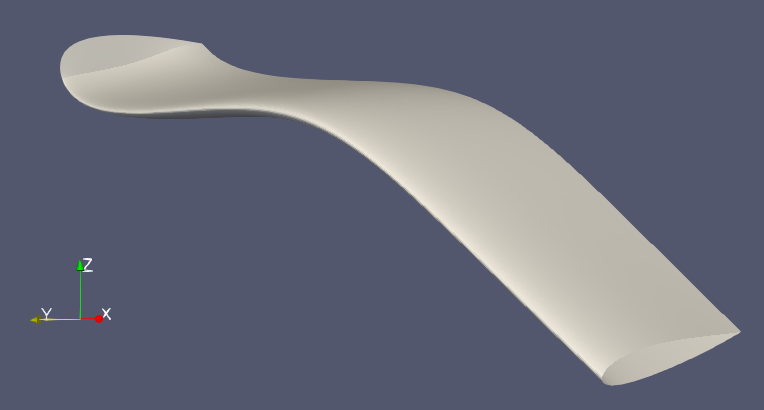
\includegraphics[scale=0.15]{figures/isoview_localwing_1.png}}
    \caption{Isometric view of local optima 1.}
    \label{isoview_localoptima_1}
\end{figure}
}
\parbox{0.47\linewidth}{
\begin{figure} 
    \centering
    \framebox{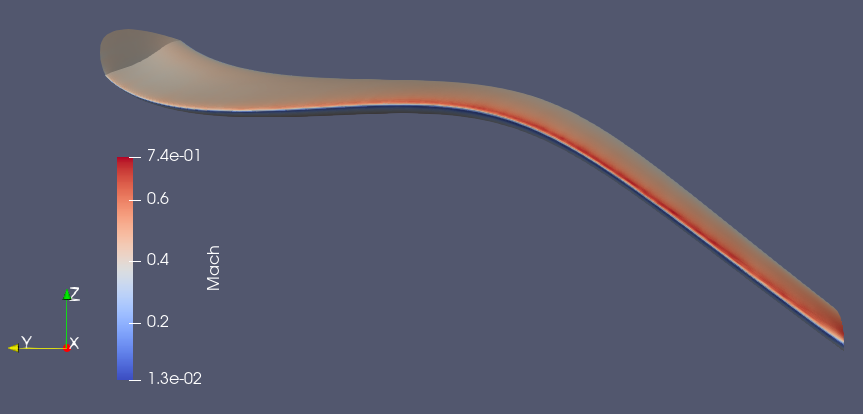
\includegraphics[scale=0.15]{figures/frontview_localwing_1.png}}
    \caption{Leading edge view of local optima 1.}
    \label{frontview_localoptima_1}
\end{figure}
}
\begin{figure} 
  \parbox{0.47\linewidth}{
    \centering
    \framebox{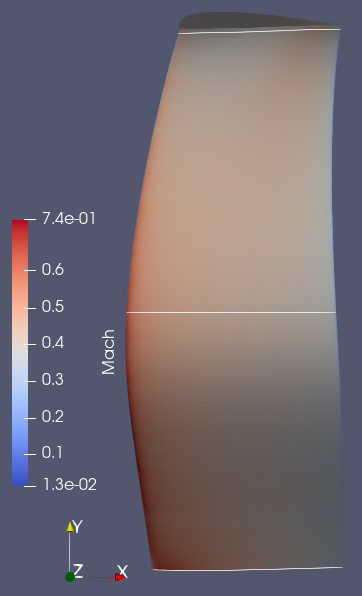
\includegraphics[scale=0.3]{figures/local_wing_1_span.png}}
    }
  \parbox{0.47\linewidth}{
    \centering
    \framebox{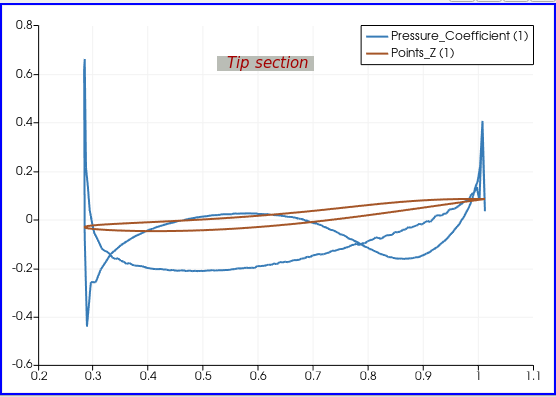
\includegraphics[scale=0.15]{figures/local_wing_1_tip_section.png}}
    \framebox{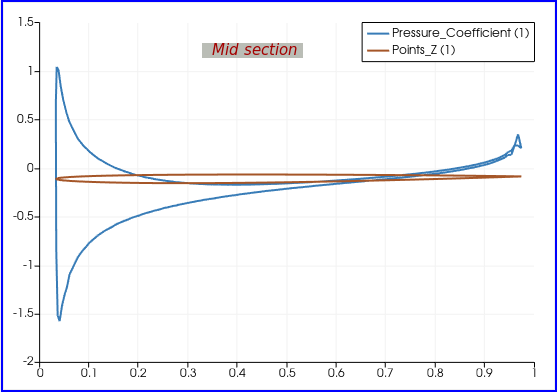
\includegraphics[scale=0.15]{figures/local_wing_1_mid_section.png}}
    \framebox{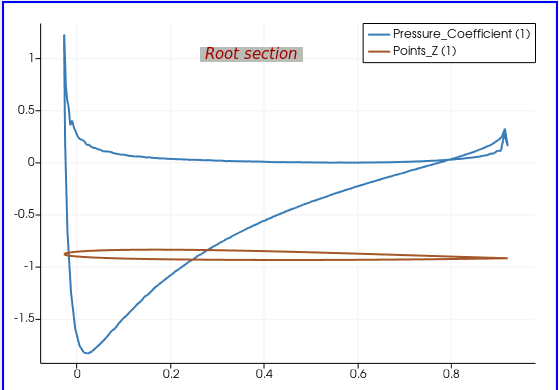
\includegraphics[scale=0.15]{figures/local_wing_1_root_section.png}}
    }
    \caption{Cp distribution at various sections in local optima 1 along span directions.}
    \label{cp_curve in span direction}
\end{figure}
\begin{itemize}
\item At root section, near the leading edge, there is a
sharp decline in Cp value in the upper surface.
\item At the tip section, the results got disrupted entirely.
\item The airfoil is highly perturbed, resulting in negative lift.
\end{itemize}

\underline{Discussion:}
\begin{itemize}
\item The sole issue for incorrect results was inadequate volume mesh points generated by glyph script.
\item Glyph script cannot be corrected remotely.
\item Also, at some sections in the optimal
wings, inverted airfoils are generated.
\end{itemize}
Assuming that the CFD solution are correct.
\begin{table}[!htbp]
    \centering
    \begin{tabular}{|c|c|c|c|c|c|c|}\hline
          & $C_l$ & $C_d$ & $C_{M_x}$ & $AoA$ & Span & Obj.diff \\\hline
        local optima 1 & 0.2625 & 0.01120   & 0.1038 & 5.535$^0$ & 2.779 & 0.0\%\\
        local optima 2 & 0.2625 & 0.01203   & 0.1005 & 3.213$^0$ & 2.918 & 7.4\%\\
        local optima 3 & 0.2625 & 0.01204   & 0.1028 & 1.972$^0$ & 2.726 & 7.5\%\\
        local optima 4 & 0.2625 & 0.01215   & 0.998  & 2.774$^0$ & 3.291 & 8.4\%\\ \hline
    \end{tabular}
    \caption{$C_d$ values for various local optima.}
    \label{optimal shape}
\end{table}

\begin{figure} 
    \centering
    \framebox{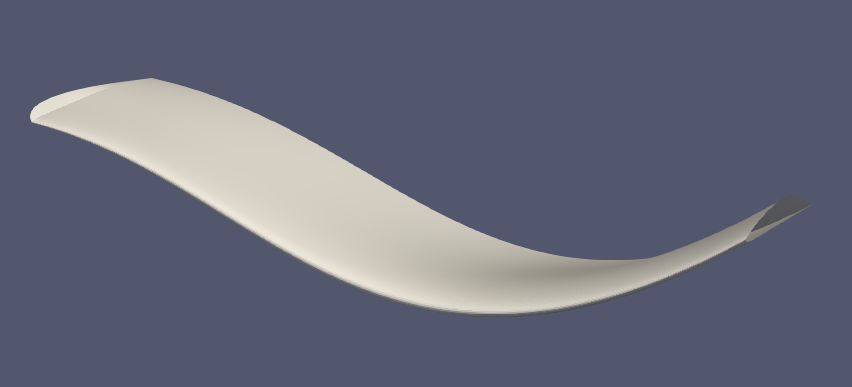
\includegraphics[scale=0.23]{figures/wing_13_iso.png}}
    \caption{Local optima 2}
    \label{local optima 2}
\end{figure}

\begin{figure} 
    \centering
    \framebox{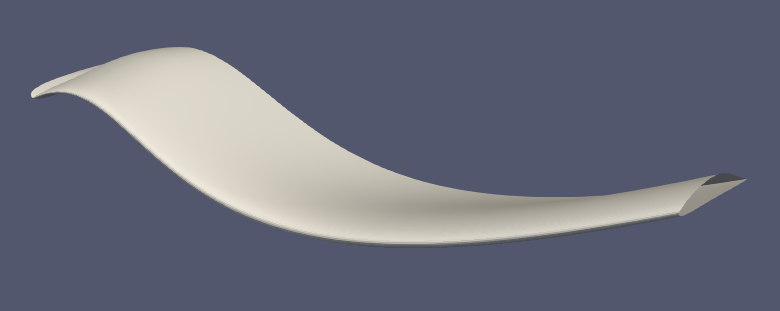
\includegraphics[scale=0.23]{figures/wing_20_iso.png}}
    \caption{Local optima 3}
    \label{local optima 3}
\end{figure}

\begin{figure}
    \centering
    \framebox{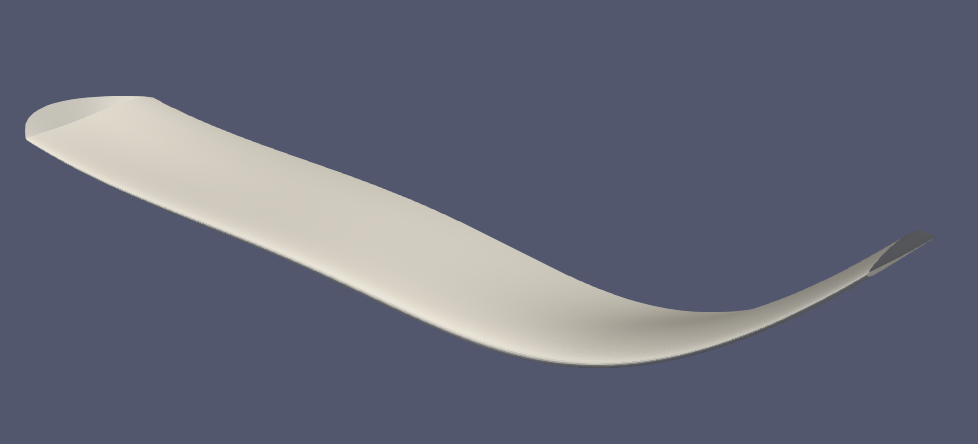
\includegraphics[scale=0.2]{figures/wing_14_iso.png}}
    \caption{Local optima 4}
    \label{local optima 4}
\end{figure}

\underline{Future work:}
\begin{itemize}
\item Additional work is necessary to improve the
performance of glyph script. 
\item The choice of design space needs to be examined.
\item Reducing
the number of CFD runs will significantly reduce the time taken for full optimization.
\item Existence of multimodality in viscous flow need to be examined.
\end{itemize}

\end{frame}